\beginsong{Der Wagen}[
    mel={Sergej Kossigin}, 
    txt={fotler (Erik Schellhorn), Igor Plachonin}, 
    index={Staub, Staub und Steppenland}, 
    index={Wagen, Der}, 
    siru={222}, 
    biest={630},
    buedel={281},
]

\renewcommand{\everychorus}{\textnote{\bf Zwischenspiel}}
\beginchorus
\endchorus
\includegraphics[draft=false, page=1]{Noten/Wagen-Zwischenspiel.pdf}	

\beginverse
\endverse
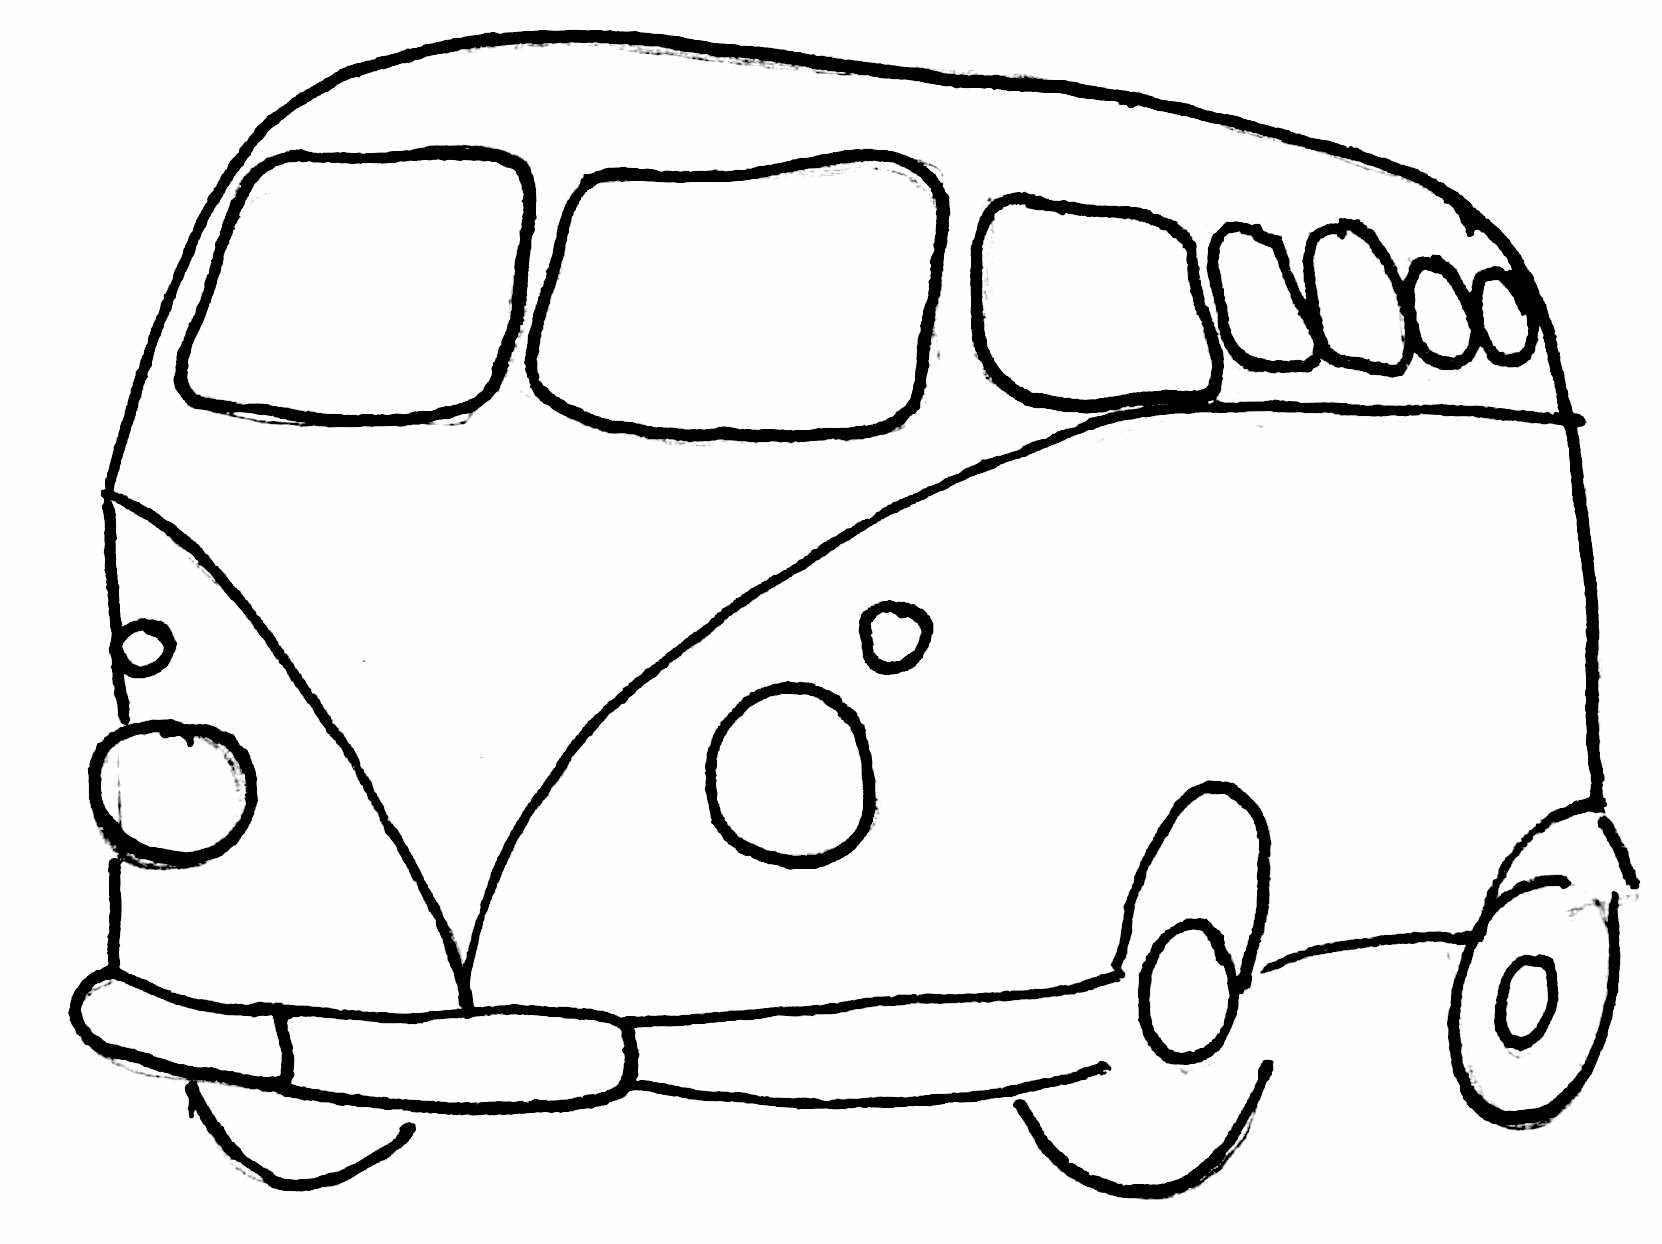
\includegraphics[draft=false, page=1]{Noten/Wagen.pdf}


% \beginverse\memorize
% \[Am]Staub, \[F]Staub \[G]und Steppen\[Am]land,
% zwei alte \[F]Mulis\[G] am Weges\[Am]rand.
% Zieh'n den \[F]Wagen\[G] aus der \[Dm]Stadt,
% weiter nach \[Am]Osten\[E] dreht sich das \[Am]Rad.
% \endverse

\beginverse\memorize
\[Am]Glaub', \[F]glaub',\[G] mein alter \[Am]Freund, 
vom Glück da \[F]haben\[G] wir oft ge\[Am]träumt. 
Knarrt das \[F]Fuhrwerk\[G] im Sturmge\[Dm]braus, 
die Mulis \[Am]finden\[E]{ nie} mehr nach \[Am]Haus.
\endverse

\beginverse
^Fern, ^fern^ in schwerer ^Stund', 
hilft nur die ^Kneipe^ am Wiesen^grund.
Die Wahrheit ^ände^rn wir nie^mals, 
dem Schicksal ^trotzend^{ auf} weiter ^Straß'.
\endverse

\beginverse
^Weit, ^weit^ und grau der ^Weg 
und unsre ^Stiefel^ steh'n starr vor ^Dreck. 
Die Fahrt vor^bei^, in Träumen ^zieh'n 
wir im ^Wagen^ nochmals da^hin.
\endverse

\beginverse
^Staub, ^Staub^ und Steppen^land,
zwei alte ^Mulis^ am Weges^rand,
zieh'n den ^Wagen^ aus der ^Stadt,
weiter nach ^Osten^ dreht sich das ^Rad.
\endverse

\beginverse
^Stjep, ^Stjep^, Stjep kru^gom, 
dwa starich ^mula^ vesut fur^gon. 
Iz gorodor ^ot^ suje^ti 
na Dalni ^zapad^ uchodim ^my.
\endverse

\endsong
